\chapter{Προτεινόμενος Περιγραφέας} \label{chap:sug}
Το εγχείρημα της παρούσας διπλωματικής εργασίας είναι η δημιουργία μίας αναπαράστασης εικόνας, η οποία παραμένει αναλλοίωτη σε μετασχηματισμούς της εικόνας, όπως περιστροφή, κλιμάκωση ή/και μετατόπιση και μπορεί να χρησιμοποιηθεί ως τοπικός περιγραφέας υφής. Η προτεινόμενη υλοποίηση σχεδιάστηκε έτσι, ώστε να εκμεταλλεύεται τη δομή και τις ιδιότητες των συσχετίσεων τρίτης τάξης (Κεφ. \ref{chap:correlations}).
\section{Θεωρητική Ανάλυση της Αναπαράστασης} \label{chap:theor}
\paragraph*{}
Έστω διδιάστατο σήμα $x(\textbf{t})$ και η τρίτης τάξης συσχέτισή του $x_3(\boldsymbol{\tau_1},\boldsymbol{\tau_2})$, της οποίας οι δείκτες $(\boldsymbol{\tau_1},\boldsymbol{\tau_2})$ είναι δυο διδιάστατα διανύσματα που εκτείνονται σε όλο το $S'=[-(N-1), \cdots ,N-1]\times[-(N-1), \cdots ,N-1]$. Για κάθε $(\boldsymbol{\tau_1},\boldsymbol{\tau_2})$, μπορεί να οριστεί ένα νοητό τρίγωνο πάνω στο  $x(\textbf{t})$. Οι κορυφές του τριγώνου συμπίπτουν με τρία στοιχεία του σήματος. Αν το τρίγωνο αυτό μετακινηθεί, χωρίς να αλλάξει το μέγεθος και ο προσανατολισμός του, σε όλες τις δυνατές θέσεις πάνω στο σήμα και σε καθεμία διαφορετική θέση (συμπεριλαμβανόμενης και της αρχικής) υπολογισθεί το γινόμενο των εκάστοτε στοιχείων των κορυφών και, στο τέλος, αθροιστούν όλα τα γινόμενα, τότε έχουμε την τιμή $x_3(\boldsymbol{\tau_1},\boldsymbol{\tau_2})$.
\paragraph*{}
Ορίζεται, έτσι, το σύνολο $W(\boldsymbol{\tau_1},\boldsymbol{\tau_2})$, το οποίο περιέχει όλα τα τρίγωνα που δημιουργήθηκαν από τις επανατοποθετήσεις του αρχικού τριγώνου $(\boldsymbol{\tau_1},\boldsymbol{\tau_2})$. Ορίζεται, επίσης, το σύνολο $K(\boldsymbol{\tau_1},\boldsymbol{\tau_2})$, το οποίο περιέχει όλα τα τρίγωνα που είναι \textit{όμοια}\footnote{Δύο τρίγωνα χαρακτηρίζονται ως όμοια, αν κάθε γωνία του ενός τριγώνου έχει το ίδιο μέτρο με την αντίστοιχη γωνία στο άλλο τρίγωνο, ή, ισοδύναμα, αν ο λόγος των μηκών των πλευρών τους είναι ίδιος και για τις τρεις πλευρές.}  με αυτά του συνόλου $W(\boldsymbol{\tau_1},\boldsymbol{\tau_2})$. Στη συνέχεια, για κάθε σύνολο $K(\boldsymbol{\tau_1},\boldsymbol{\tau_2})$ αντιστοιχίζεται μία κλάση $C(\boldsymbol{\tau_1},\boldsymbol{\tau_2})$ με στοιχεία της συσχέτισης. Κάθε κλάση $C(\boldsymbol{\tau_1},\boldsymbol{\tau_2})$ περιέχει όλα εκείνα τα στοιχεία της συσχέτισης, των οποίων οι δείκτες δημιουργούν τρίγωνα όμοια με το αρχικό τρίγωνο των διανυσμάτων $(\boldsymbol{\tau_1},\boldsymbol{\tau_2})$.

\paragraph*{}
Έχοντας στην κατοχή μας τα νεοσυσταθέντα σύνολα και κλάση, παρατηρούμε πως, για διαφορετικούς δείκτες $(\boldsymbol{\tau_1},\boldsymbol{\tau_2})$ και $(\boldsymbol{\tau_1}',\boldsymbol{\tau_2}')$, μπορούν να δημιουργηθούν πανομοιότυπες κλάσεις $C(\boldsymbol{\tau_1},\boldsymbol{\tau_2})$ και $C(\boldsymbol{\tau_1}',\boldsymbol{\tau_2}')$, είτε γιατί τα $(\boldsymbol{\tau_1},\boldsymbol{\tau_2})$ και $(\boldsymbol{\tau_1}',\boldsymbol{\tau_2}')$ δημιουργούν όμοια αρχικά τρίγωνα, είτε γιατί πολλά στοιχεία της συσχέτισης είναι ίσα, λόγω των συμμετριών που ισχύουν (εξ. \ref{eq:symmetries}). Προκειμένου να αποφευχθεί αυτή η κατάσταση, δημιουργούμε τις κλάσεις $C(\boldsymbol{\tau_1},\boldsymbol{\tau_2})$ κρατώντας σταθερό το $\boldsymbol{\tau_1}$ στη θέση $\boldsymbol{\tau_1} = [1,0]$ και επιτρέποντας στο $\boldsymbol{\tau_2}$ να παίρνει τιμές από το υποσύνολο $S_0 \triangleq [1,0]\times[0,\infty]$.

\paragraph*{}
Αφού έχει εξασφαλισθεί πως οι κλάσεις $C(\boldsymbol{\tau_1},\boldsymbol{\tau_2})$ δεν περιέχουν επαναλαμβανόμενα στοιχεία, βλέπουμε πως οποιαδήποτε αλλαγή του $x(\textbf{t})$ (περιστροφή ή κλιμάκωση) οδηγεί σε επανατοποθέτηση των στοιχείων της κάθε κλάσης $C(\boldsymbol{\tau_1},\boldsymbol{\tau_2})$ μέσα στην ίδια κλάση, ενώ οι κλάσεις ως σύνολα δεν αλλάζουν και συνεχίζουν να περιέχουν τα ίδια στοιχεία. Έτσι, ορίζεται η παρακάτω αναπαράσταση για τα στοιχεία της κάθε κλάσης:
\begin{equation}\label{eq:x3tilde}
\tilde{x_3}(\rho,\phi;\boldsymbol{\tau_1},\boldsymbol{\tau_2}) \triangleq x_3(\textbf{T}_{\beta,\phi}\boldsymbol{\tau_1},\textbf{T}_{\beta,\phi}\boldsymbol{\tau_2})
\end{equation}
όπου,
\begin{equation}
\textbf{T}_{\beta,\phi} = \beta\begin{bmatrix} \cos\phi & -\sin\phi \\ \sin\phi & \cos\phi \end{bmatrix} \text{ και } \rho = \log\beta \nonumber
\end{equation}
Εισάγονται οι μεταβλητές $\rho \text{ και } \phi$ για να αναπαρασταθούν όλα τα τρίγωνα της κλάσης $C(\boldsymbol{\tau_1},\boldsymbol{\tau_2})$, τα οποία έχουν υποστεί συστολή/διαστολή $\beta$ ή/και περιστροφή κατά γωνία $\phi$.

\paragraph*{}
Αν θεωρηθεί λοιπόν το σήμα $y(\textbf{t}) = x(\textbf{T}_{\alpha,\theta}\textbf{t}+\textbf{t}_0)$, τότε στο εσωτερικό κάθε κλάσης $C(\boldsymbol{\tau_1},\boldsymbol{\tau_2})$ η αναπαράστασή του γίνεται:
\begin{equation}
\tilde{y_3}(\rho,\phi;\boldsymbol{\tau_1},\boldsymbol{\tau_2}) = \tilde{x_3}(\rho+\log\alpha,\phi+\theta;\boldsymbol{\tau_1},\boldsymbol{\tau_2})
\end{equation}

\paragraph*{}
Στη συνέχεια, από την αναπαράσταση του $\tilde{x_3}$, υπολογίζεται ο διδιάστατος μετασχηματισμός Fourier ως προς τις μεταβλητές $\rho \text{ και } \phi$, προκειμένου να αποβληθεί η επιρροή του παράγοντα περιστροφής ή/και κλιμάκωσης. Πλέον έχει παραχθεί το $\tilde{X_3}(P,\Phi;\boldsymbol{\tau_1},\boldsymbol{\tau_2})$. Παράλληλα, γίνονται κάποιες αλλαγές και ενέργειες, προκειμένου να προκύψει μια αντιπροσωπευτική αναπαράσταση του σήματος, η οποία είναι όσο πιο οικονομική γίνεται, από άποψη όγκου δεδομένων αλλά και από άποψη υπολογιστικών απαιτήσεων για τη δημιουργία της.

\paragraph*{}
Η πρώτη ενέργεια για την επίτευξη των παραπάνω είναι το να συμπεριληφθεί στην τελική αναπαράσταση μόνο το πλάτος του μετασχηματισμού $\tilde{X_3}(P,\Phi;\boldsymbol{\tau_1},\boldsymbol{\tau_2})$ και όχι φάση του. Επίσης μία επιπλέον επιλογή είναι να κρατηθεί μόνο η μηδενική συχνότητα του πλάτους. Υπολογίζεται, δηλαδή το $\abs{\tilde{X_3}(0,0;\boldsymbol{\tau_1},\boldsymbol{\tau_2})}$. Στη συνέχεια υιοθετείται μία καινούρια έκφραση για τους δείκτες $(\boldsymbol{\tau_1},\boldsymbol{\tau_2})$. Αντί για δύο διανύσματα $\boldsymbol{\tau_1}=[\tau_{1x}, \tau_{1y}]$ και $\boldsymbol{\tau_2}=[\tau_{2x}, \tau_{2y}]$, μπορεί να χρησιμοποιηθεί ένα από παρακάτω συστήματα:
\begin{enumerate}
\item
$(\boldsymbol{\tau_1},\boldsymbol{\tau_2}) = (\boldsymbol{\tau_0},[k,l]), k\in[0,1], l\in[0,\infty]$
\item
$(\boldsymbol{\tau_1},\boldsymbol{\tau_2}) = (\boldsymbol{\tau_0},\boldsymbol{\tau_2})\rightarrow(\theta_1,\theta_2), \theta_1,\theta_2\in\left[0,\dfrac{\pi}{2}\right]$
\item
$(\boldsymbol{\tau_1},\boldsymbol{\tau_2}) = (\boldsymbol{\tau_0},\boldsymbol{\tau_2})\rightarrow(\theta_1,\lambda), \theta_1\in\left[0,\dfrac{\pi}{2}\right], \lambda\in[0,\infty]$
\end{enumerate}
όπου $\boldsymbol{\tau_0} = (1,0)$, οι $\theta_1, \theta_2$ είναι οι γωνίες των διανυσμάτων $(\boldsymbol{\tau_1},\boldsymbol{\tau_2})$ και $(\boldsymbol{\tau_1},\boldsymbol{\tau_2}-\boldsymbol{\tau_1})$ αντίστοιχα και $\lambda$ είναι ο λόγος $\dfrac{\abs{\boldsymbol{\tau_1}}}{\abs{\boldsymbol{\tau_2}}}$. Σε όλες τις παραπάνω περιπτώσεις ο τετραδιάστατος χώρος, που εκφράζεται από τα $(\boldsymbol{\tau_1},\boldsymbol{\tau_2})$, μειώνεται αισθητά σε ένα διδιάστατο χώρο, χωρίς καθόλου απώλεια πληροφορίας.\\
Στην παρούσα διπλωματική εργασία έχει υιοθετηθεί το δεύτερο σύστημα, το οποίο φαίνεται γραφικά στο Σχήμα \ref{fig:theta1theta2}.

\begin{figure}
\begin{center}
\psscalebox{1.5 1.5} % Change this value to rescale the drawing.
{
\begin{pspicture}(2.7,-3.0179136)(10,1.0179136)

\psline[linecolor=black, linewidth=0.03, arrowsize=0.05291666666666667cm 2.0,arrowlength=1.4,arrowinset=0.0]{->}(3.9811344,-2.8214464)(8.910367,-1.362257)
\psline[linecolor=black, linewidth=0.03, arrowsize=0.05291666666666667cm 2.0,arrowlength=1.4,arrowinset=0.0]{->}(3.9811344,-2.8214464)(6.7160273,-0.58570236)
\psline[linecolor=black, linewidth=0.03, linestyle=dashed, dash=0.17638889cm 0.10583334cm](8.910367,-1.362257)(6.7160273,-0.58570236)
\psline[linecolor=black, linewidth=0.03, arrowsize=0.05291666666666667cm 2.0,arrowlength=1.4,arrowinset=0.0]{->}(4.0,-2.8)(10.8,-2.8)
\psarc[linecolor=black, linewidth=0.02, dimen=outer, arrowsize=0.05291666666666667cm 2.0,arrowlength=1.4,arrowinset=0.0]{->}(4.0,-2.8){1.2}{0.0}{25.0}
\psarc[linecolor=black, linewidth=0.02, dimen=outer, arrowsize=0.05291666666666667cm 2.0,arrowlength=1.4,arrowinset=0.0]{<-}(10.8,-2.8){1.2}{141.0}{180.0}
\psline[linecolor=black, linewidth=0.03, arrowsize=0.05291666666666667cm 2.0,arrowlength=1.4,arrowinset=0.0]{->}(4.0,-2.8)(8.4,-0.8)
\psline[linecolor=black, linewidth=0.03, linestyle=dashed, dash=0.17638889cm 0.10583334cm](10.8,-2.8)(8.4,-0.8)
\psline[linecolor=black, linewidth=0.04, arrowsize=0.05291666666666667cm 2.0,arrowlength=1.4,arrowinset=0.0]{->}(4.0,-2.8)(11.6,-2.8)
\psline[linecolor=black, linewidth=0.04, arrowsize=0.05291666666666667cm 2.0,arrowlength=1.4,arrowinset=0.0]{->}(4.0,-2.8)(4.0,0.4)
\psarc[linecolor=black, linewidth=0.02, dimen=outer, arrowsize=0.05291666666666667cm 2.0,arrowlength=1.4,arrowinset=0.0]{->}(4.0,-2.8){1.6}{16.0}{39.0}
\psarc[linecolor=black, linewidth=0.02, dimen=outer, arrowsize=0.05291666666666667cm 2.0,arrowlength=1.4,arrowinset=0.0]{<-}(8.8,-1.2){1.2}{166.0}{206.0}
\psarc[linecolor=black, linewidth=0.02, dimen=outer, arrowsize=0.05291666666666667cm 2.0,arrowlength=1.4,arrowinset=0.0]{->}(4.0,-2.8){2.4}{0.0}{16.0}
\rput[bl](9.6,-3.2){$\tau_0 \equiv \tau_1$}
\rput[bl](6.8,-2.8){$\phi$}
\rput[bl](5.6,-2.8){$\theta_1$}
\rput[bl](5.6,-2.0){$\theta_1$}
\rput[bl](9.2,-2.4){$\theta_2$}
\rput[bl](7.2,-1.2){$\theta_2$}
\rput[bl](8.0,-0.8){$\tau_2$}
\rput[bl](8.4,-2.0){$\tau_1'$}
\rput[bl](6.0,-0.8){$\tau_2'$}
\rput[bl](4.4,0.0){$\rho = \log \frac{|\tau_1'|}{|\tau_0|}$}
\end{pspicture}

}
\end{center}
\caption{Σύστημα Αναπαράστασης Διανυσμάτων με τις γωνίες $\theta_1,\theta_2$.}
  \label{fig:theta1theta2}
\end{figure}


\paragraph*{}
Είναι σημαντικό να σημειωθεί, ότι κατά τον υπολογισμό των μεταβλητών $\rho$, $\phi$, $\theta_1$ και $\theta_2$, επειδή οι τιμές τους είναι πολύ πιθανό να είναι πραγματικοί αριθμοί, υπόκεινται σε κβάντιση, προκειμένου να μπορούν να αντιστοιχηθούν ένα διακριτό πλέγμα. Ο βέλτιστος αριθμός επιπέδων κβάντισης για την κάθε μεταβλητή είναι ένας προβληματισμός, ο οποίος πρέπει να μελετηθεί στο πειραματικό στάδιο.

\paragraph*{}
Επίσης σημαντικό είναι, το γεγονός ότι, το $\tilde{x_3}(\rho,\phi;\boldsymbol{\tau_1},\boldsymbol{\tau_2})$ δεν υπολογίζεται απευθείας από την εξίσωση \ref{eq:x3tilde}. Αντί να υπολογισθεί το $x_3(\textbf{T}_{\beta,\phi}\boldsymbol{\tau_1},\textbf{T}_{\beta,\phi}\boldsymbol{\tau_2})$ για κάθε $\rho,\phi$, υπολογίζεται πρώτα το $x_3(\boldsymbol{\tau_1},\boldsymbol{\tau_2})$ και μετά η τιμή που υπολογίσθηκε αντιστοιχίζεται σε κάποια $\rho,\phi$. Επίσης η τιμή αντιστοιχίζεται σε κάποια κλάση, ανάλογα με το ποιο από τα τρία προαναφερθέντα συστήματα χρησιμοποιείται. Έτσι, τελικά προστίθεται αυτή η τιμή στο κατάλληλο στοιχείο του $\tilde{x_3}$. Επιπλέον, για κάθε $\boldsymbol{\tau_1}\in S'$, το $\boldsymbol{\tau_2}$ δε χρειάζεται να παίρνει τιμές από όλο το $S'$. Για την ακρίβεια, μπορεί να παίρνει τιμές από το:
\begin{equation}
S''(\boldsymbol{\tau_1}) = \lbrace  \boldsymbol{\tau_2} \in S': 0 \leq \boldsymbol{\tau_1} \cdot \boldsymbol{\tau_2} \leq \abs{ \boldsymbol{\tau_1}}^2 , 0 \leq \boldsymbol{\tau_1} \cdot \boldsymbol{\tau_2}', (\boldsymbol{\tau_1}-\boldsymbol{\tau_2})\in S' \rbrace
\end{equation}
όπου το $\boldsymbol{\tau_2}'$ είναι το διάνυσμα $\boldsymbol{\tau_2}$ περιστραμμένο με την ωρολογιακή φορά κατά 90 μοίρες. Το παραπάνω σύνολο $S''(\boldsymbol{\tau_1})$ προκύπτει αν λάβουμε υπόψιν τις συμμετρίες των συσχετίσεων (προκύπτουν οι δύο πρώτοι περιορισμοί) και το γεγονός ότι το $x_3(\boldsymbol{\tau_1},\boldsymbol{\tau_2})$ είναι μηδέν όταν $(\boldsymbol{\tau_1}-\boldsymbol{\tau_2})\not\in S'$. Ο περιορισμός αυτός του $\boldsymbol{\tau_2}$ απλοποιεί σε πολύ μεγάλο βαθμό την υπολογιστική διαδικασία.

\paragraph*{}
Τελικά το $\abs{\tilde{X_3}(0,0;\theta_1,\theta_2)}$, αποτελεί τον τοπικό περιγραφέα της γειτονιάς, η οποία έχει τροφοδοτηθεί στον αλγόριθμο. 

% =========================================================================================================================
% =========================================================================================================================

\section{Αλγοριθμική Υλοποίηση της Αναπαράστασης}
\paragraph*{}
Σε αυτή την ενότητα παρατίθενται οι αλγοριθμικές μορφές της υλοποίησης της αναπαράστασης και του υπολογισμού της συσχέτισης τρίτου βαθμού μιας εικόνας.\\


\begin{algorithm}
\caption{Υπολογισμός αμετάβλητης αναπαράστασης εικόνας.}
\label{alg:imRep}
\begin{algorithmic}[1]
\STATE variable initialization;
\STATE calculate $\max(\rho),\max(\phi)$ for quantization;
\STATE $x_3 \gets 3rdOrderCorrelationOf(x)$;
\FOR{$\boldsymbol{\tau_1} \in S'$}
	\FOR{$\boldsymbol{\tau_2} \in S''(\boldsymbol{\tau_1})$}
		\STATE calculate \& quantize $\rho,\phi$ by comparing $\boldsymbol{\tau_1}$ with $\boldsymbol{\tau_0} = [1,0]$;
		\STATE calculate \& quantize included angles $\theta_1,\theta_2$;
		\STATE $\tilde{x_3}(\rho,\phi;\theta_1,\theta_2) \gets \tilde{x_3}(\rho,\phi;\theta_1,\theta_2) + x_3(\boldsymbol{\tau_1},\boldsymbol{\tau_2})$;
	\ENDFOR
\ENDFOR
\STATE $\tilde{X_3}(\rho,\phi;\theta_1,\theta_2) \gets FFTAlongFirstTwoDimensionsOf(\tilde{x_3}(\rho,\phi;\theta_1,\theta_2)$
\STATE $Representation \gets \abs{\tilde{X_3}(0, 0;\theta_1,\theta_2)}$
\end{algorithmic}
\end{algorithm}


\begin{algorithm}
\caption{Υπολογισμός τρίτης τάξης συσχέτισης εικόνας.}
\label{alg:dft23}
\begin{algorithmic}[1]
\STATE variable initialization;
\STATE $X \gets FFT2Of(x)$;
\FOR{$\boldsymbol{\tau_1} \in S'$}
	\FOR{$\boldsymbol{\tau_2} \in S'$}
		\STATE $X_3(\boldsymbol{\tau_1}, \boldsymbol{\tau_2}) \gets X(\boldsymbol{\tau_1}) X(\boldsymbol{\tau_2}) X^*(\boldsymbol{\tau_1} + \boldsymbol{\tau_2})$
	\ENDFOR
\ENDFOR
\STATE $x_3 \gets iFFTnOf(X_3)$
\end{algorithmic}
\end{algorithm}

% =========================================================================================================================
% =========================================================================================================================



\section{Πολυπλοκότητα}
Ένα πολύ σημαντικό ζήτημα που πρέπει να αναλυθεί έχει να κάνει με την πολυπλοκότητα του αλγόριθμου που υλοποιήθηκε καθώς και με το χρόνο που απαιτείται για την παραγωγή μιας αναπαράστασης. Από τους αλγόριθμους της προηγούμενης ενότητας, φαίνεται, πως την πολυπλοκότητα καθορίζουν ο υπολογισμός της συσχέτισης, ο μετασχηματισμός Fourier, καθώς και οι δύο επαναληπτικοί βρόχοι.

\paragraph*{}
Από τον Αλγόριθμο \ref{alg:dft23} μπορεί να υπολογισθεί η πολυπλοκότητα του υπολογισμού της συσχέτισης. Για το μετασχηματισμό Fourier (fft), τόσο τον ευθύ, όσο και τον αντίστροφο, γνωρίζουμε πως έχει πολυπλοκότητα $O(NlogN)$. Έπειτα, είναι οι δύο επαναληπτικοί βρόχοι, προκειμένου τα $(\boldsymbol{\tau_1}, \boldsymbol{\tau_2})$ να καλύψουν όλο το $S'=[-(N-1), \cdots ,N-1]\times[-(N-1), \cdots ,N-1]$, όπου $N$, το μέγεθος της εικόνας εισόδου. Στην ουσία ο κάθε επαναληπτικός βρόχος είναι δύο εμφωλευμένοι βρόχοι, όπου αν θεωρήσουμε πως τα $(\boldsymbol{\tau_1}, \boldsymbol{\tau_2})$ είναι διανύσματα δύο διαστάσεων, τότε η κάθε συνιστώσα τους εκτείνεται σε εύρος $[-(N-1), \cdots ,N-1]$.  Υπάρχουν δηλαδή, τέσσερις επαναληπτικοί βρόχοι, ο καθένας από τους οποίους έχει $2N - 1$ επαναλήψεις. Άρα τελικά, εκτελούντα $(2N - 1)\times(2N - 1)\times(2N - 1)\times(2N - 1) = 16N^4 - 32N^3 + 24N^2 - 8N + 1$ επαναλήψεις, δηλαδή μιλάμε για πολυπλοκότητα $O(N^4)$ για τους επαναληπτικούς βρόχους, αλλά και για τον αλγόριθμο υπολογισμού της συσχέτισης συνολικά.

\paragraph*{}
Επιστρέφοντας στον Αλγόριθμο \ref{alg:imRep}, φαίνεται πως οι δύο ακόμα επαναληπτικοί βρόχοι δίνουν μια πολυπλοκότητα $O(N^4)$, η οποία υπερισχύει της πολυπλοκότητας του fft $O(NlogN)$. Θα πρέπει να σημειωθεί, βέβαια, πως στην περίπτωση του fft του βήματος (11), το ρόλο του $N$ παίζουν οι παράμετροι $(\theta_1, \theta_2)$, αφού υπολογίζοντας το μετασχηματισμό Fourier του $\tilde{x}_3(\rho, \phi, \theta_1, \theta_2)$ για κάθε $(\rho, \phi)$, στην ουσία εκτελείται ένας διδιάστατος μετασχηματισμός Fourier σε σήμα διαστάσεων $(\theta_1 + 1)\times (\theta_2 + 1)$. Άρα τελικά για είσοδο μία εικόνα διαστάσεων $(N \times N)$, η πολυπλοκότητα για τη δημιουργία της αναπαράστασής της είναι $O(N^4)$.

\paragraph*{}
Στον Πίνακα \ref{tab:times} φαίνονται ενδεικτικά οι μέσοι χρόνοι για την παραγωγή των αναπαραστάσεων για εικόνες με μέγεθος ίδιο με αυτό που επιλέχθηκε για τα πειράματα, καθώς και για τις τιμές $(|\theta_1|, |\theta_2|)$ που χρησιμοποιήθηκαν.

\begin{table}
\caption{Χρόνοι παραγωγής της προτεινόμενης αναπαράστασης}\label{tab:times}
\centerline{ 
\begin{tabular}{c|c|c||c}
$\boldsymbol{\abs{\theta_1}, \abs{\theta_2}}$ & $\boldsymbol{Radius}$  & $\boldsymbol{N}$ & $\boldsymbol{Time (msec)}$ \\ \hline
9   &  4  &  9   &  5.851  \\
9   &  8  &  17  &  85.771 \\
10  &  4  &  9   &  5.8785 \\
10  &  8  &  17  &  86.326 \\
\end{tabular}
}
\end{table}
% =========================================================================================================================
% =========================================================================================================================

\section{Παραδείγματα}
\paragraph*{}
Σε αυτή την ενότητα παρατίθενται κάποια παραδείγματα, τα οποία, έστω και σε πρωταρχικό στάδιο, επιδεικνύουν τη λειτουργία και την ανεξαρτησία της αναπαράστασης. Συγκεκριμένα χρησιμοποιήθηκαν ως είσοδοι τεχνητές εικόνες που απεικονίζουν κάποια βασικά γεωμετρικά σχήματα. Αφού υπολογισθούν οι αναπαραστάσεις τους, τα σχήματα περιστρέφονται και υπολογίζονται οι καινούριες αναπαραστάσεις. Επίσης έγιναν και κάποιες δοκιμές ως προς τον αριθμό των επιπέδων κβάντισης των τεσσάρων μεταβλητών της αναπαράστασης.

%\newpage
\begin{figure}
        \centering
        \begin{subfigure}[t]{0.5\textwidth}
                \centerline{
\includegraphics[scale = 0.5]{./images/examples/smallerTetragwno.png}}
                \caption{Τετράγωνο}
                \label{fig:rect}
        \end{subfigure}%
        ~
        \centering
        \begin{subfigure}[t]{0.5\textwidth}
                \centerline{
\includegraphics[scale = 0.5]{./images/examples/RotatedsmallerTetragwno.png}}
                \caption{Περιστραμμένο τετράγωνο}
        \end{subfigure}%
        
        \centering
        \begin{subfigure}[b]{1\textwidth}
                \centerline{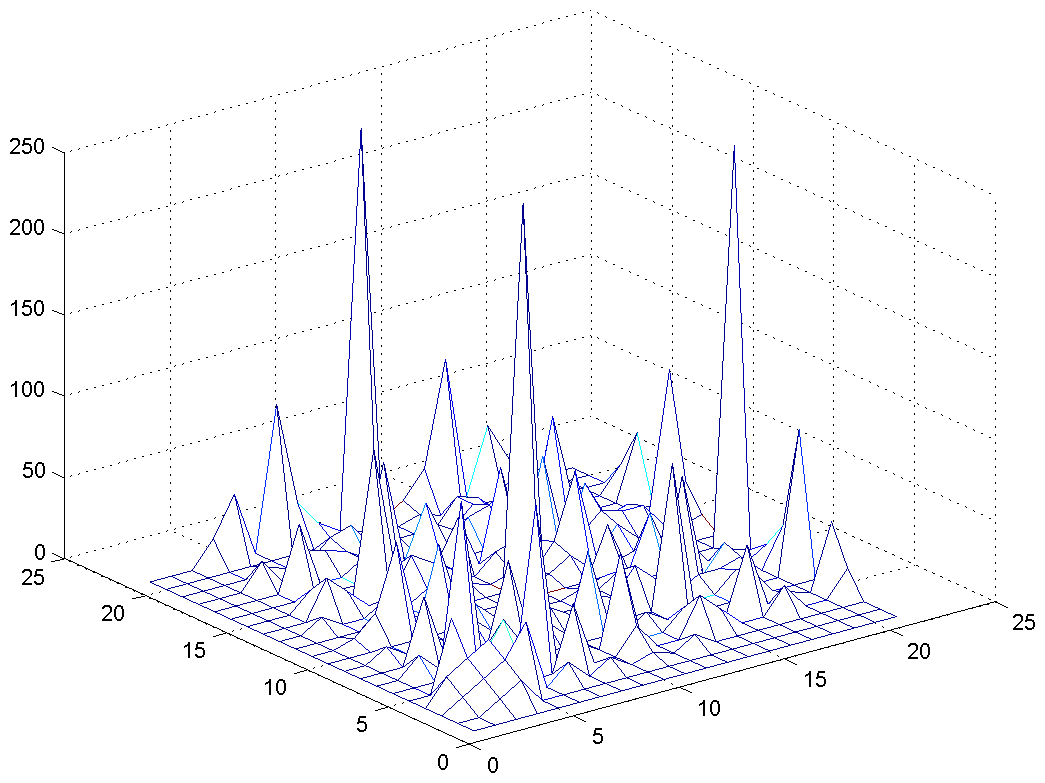
\includegraphics[scale = 0.3]{./images/examples/smallerTetragwno(15152020).png}}
                \caption{Αναπαράσταση τετραγώνου με αριθμό επιπέδων κβάντισης: $\abs{\rho} = 15,\abs{\phi} = 15,\abs{\theta_1} = 20,\abs{\theta_2} = 20$}
        \end{subfigure}%

        \centering
        \begin{subfigure}[b]{1\textwidth}
                \centerline{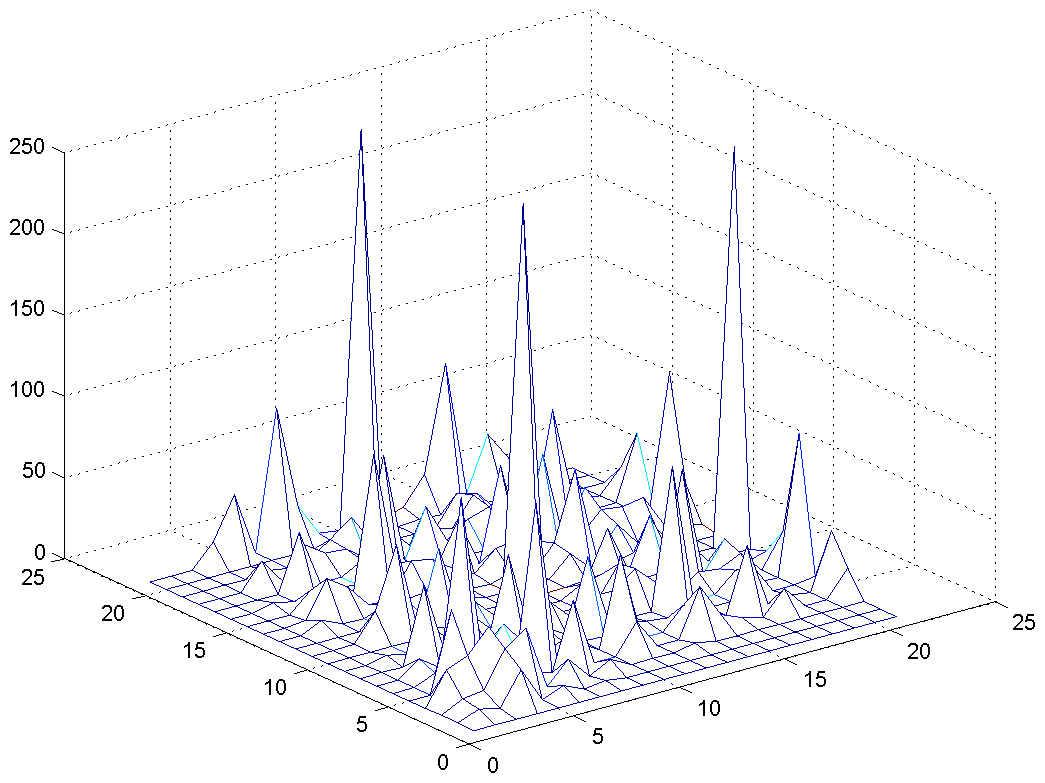
\includegraphics[scale = 0.3]{./images/examples/RotatedsmallerTetragwno(15152020).png}}
                \caption{Αναπαράσταση περιστραμμένου τετραγώνου με αριθμό επιπέδων κβάντισης: $\abs{\rho} = 15,\abs{\phi} = 15,\abs{\theta_1} = 20,\abs{\theta_2} = 20$}
        \end{subfigure}%
        \caption{Παράδειγμα με τετράγωνο}
        \label{fig:ex_rect}
\end{figure}
% =========================================================================================================================
% =========================================================================================================================

\begin{figure}
        \centering
        \begin{subfigure}[t]{0.5\textwidth}
                \centerline{
\includegraphics[scale = 0.5]{./images/examples/emptyTetragwno.png}}
                \caption{Περίγραμμα τετραγώνου}
        \end{subfigure}%
        ~
        \centering
        \begin{subfigure}[t]{0.5\textwidth}
                \centerline{
\includegraphics[scale = 0.5]{./images/examples/emptyRotatedTetragwno.png}}
                \caption{Περιστραμμένο περίγραμμα τετραγώνου}
        \end{subfigure}%

        \centering
        \begin{subfigure}[b]{1\textwidth}
                \centerline{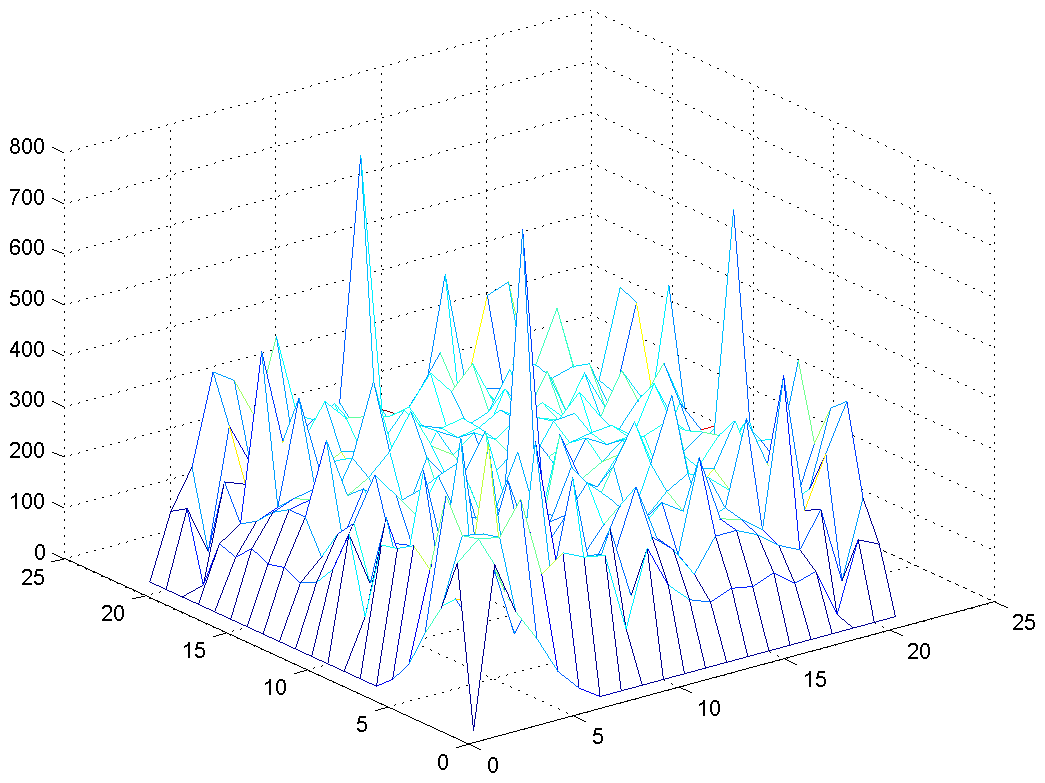
\includegraphics[scale = 0.3]{./images/examples/emptyTetragwno(15152020).png}}
                \caption{Αναπαράσταση περιγράμματος τετραγώνου με αριθμό επιπέδων κβάντισης: $\abs{\rho} = 15,\abs{\phi} = 15,\abs{\theta_1} = 20,\abs{\theta_2} = 20$}
        \end{subfigure}%

        \centering
        \begin{subfigure}[b]{1\textwidth}
                \centerline{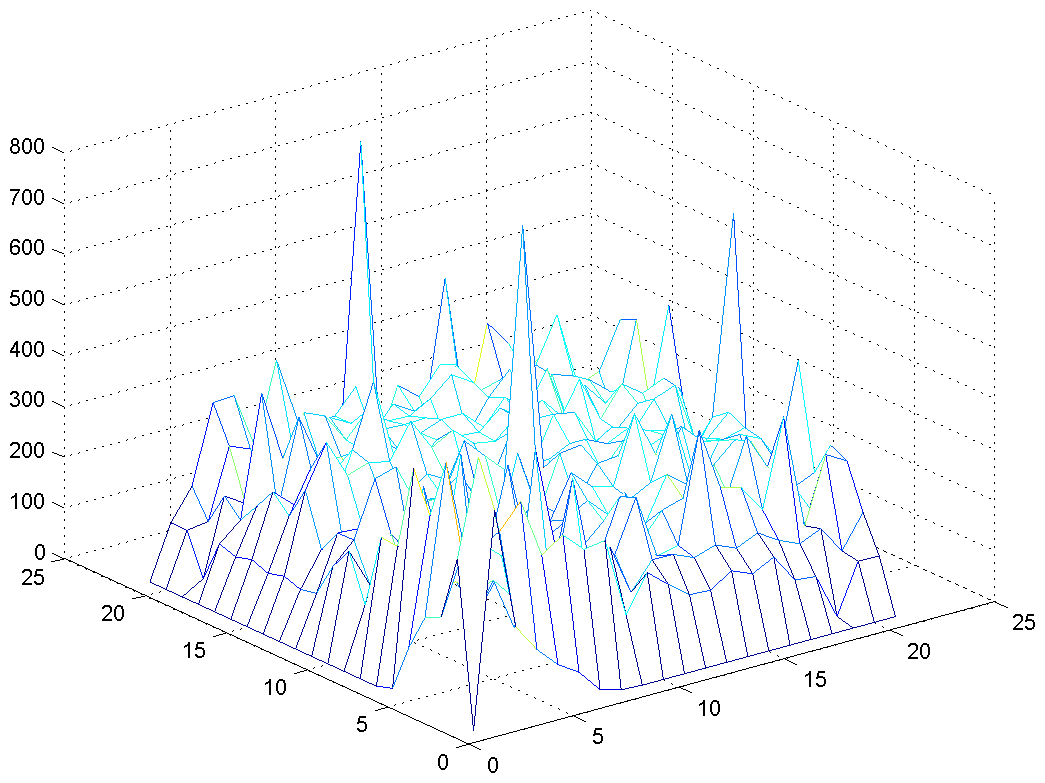
\includegraphics[scale = 0.3]{./images/examples/emptyRotatedTetragwno(15152020).png}}
                \caption{Αναπαράσταση περιστραμμένου περιγράμματος τετραγώνου με αριθμό επιπέδων κβάντισης: $\abs{\rho} = 15,\abs{\phi} = 15,\abs{\theta_1} = 20,\abs{\theta_2} = 20$}
        \end{subfigure}%
        \caption{Παράδειγμα με περίγραμμα τετραγώνου}
\end{figure}
% =========================================================================================================================
% =========================================================================================================================

\begin{figure}
        \centering
        \begin{subfigure}[t]{0.3\textwidth}
                \centerline{
\includegraphics[scale = 0.5]{./images/examples/trigwno.png}}
                \caption{Τρίγωνο}
        \end{subfigure}%
        ~
        \centering
        \begin{subfigure}[t]{0.3\textwidth}
                \centerline{
\includegraphics[scale = 0.5]{./images/examples/trigwno90.png}}
                \caption{Περιστραμμένο τρίγωνο κατά 90 μοίρες}
        \end{subfigure}%
        \centering
        \begin{subfigure}[t]{0.3\textwidth}
                \centerline{
\includegraphics[scale = 0.5]{./images/examples/Rotatedtrigwno.png}}
                \caption{Περιστραμμένο τρίγωνο}
        \end{subfigure}%

        \centering
        \begin{subfigure}[b]{1\textwidth}
                \centerline{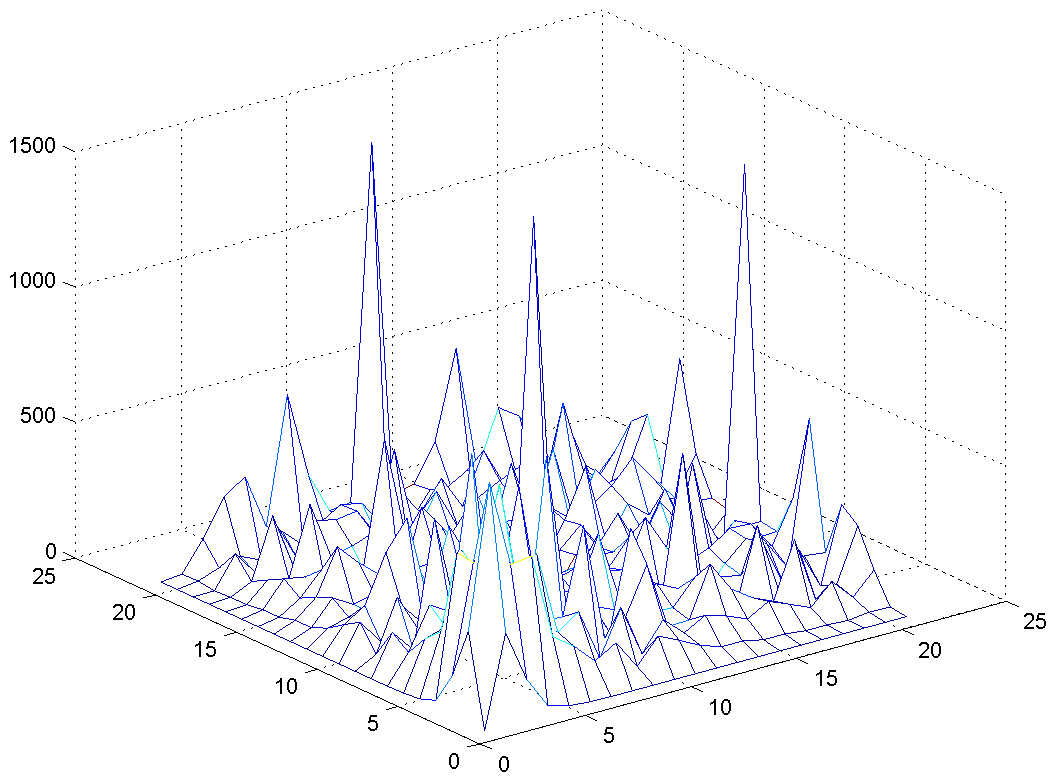
\includegraphics[scale = 0.3]{./images/examples/trigwno(15152020).png}}
                \caption{Αναπαράσταση τριγώνου με αριθμό επιπέδων κβάντισης: $\abs{\rho} = 15,\abs{\phi} = 15,\abs{\theta_1} = 20,\abs{\theta_2} = 20$}
        \end{subfigure}%

        \centering
        \begin{subfigure}[b]{1\textwidth}
                \centerline{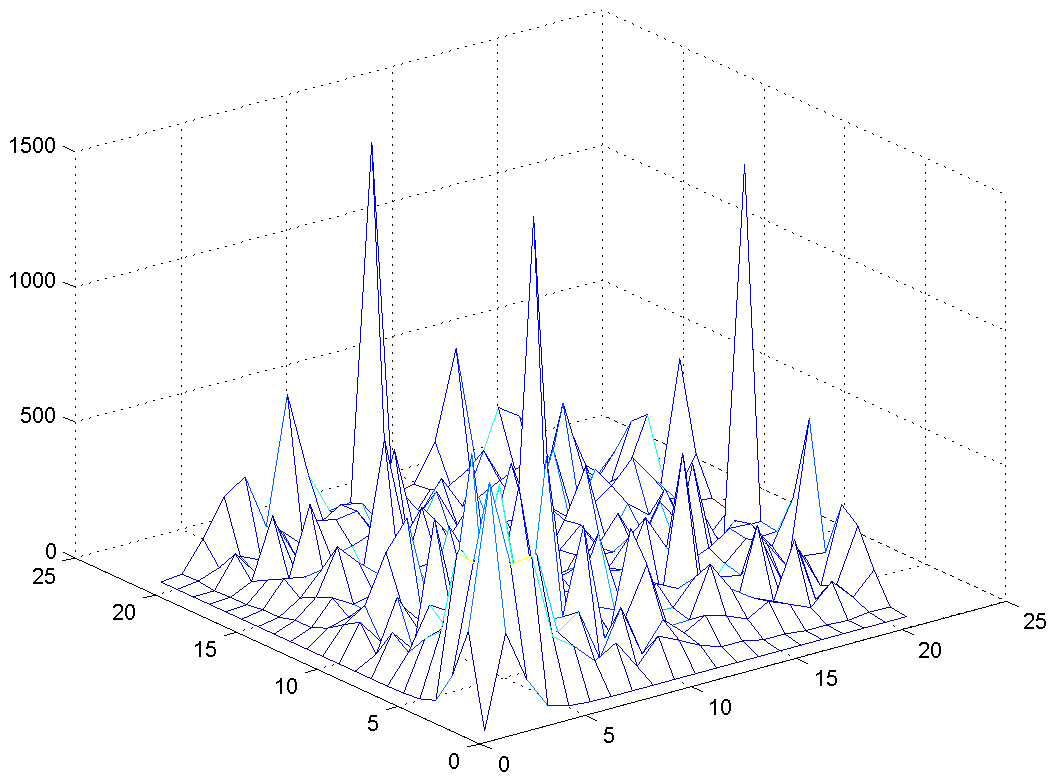
\includegraphics[scale = 0.3]{./images/examples/trigwno90(15152020).png}}
                \caption{Αναπαράσταση περιστραμμένου κατά 90 μοίρες τριγώνου με αριθμό επιπέδων κβάντισης: $\abs{\rho} = 15,\abs{\phi} = 15,\abs{\theta_1} = 20,\abs{\theta_2} = 20$}
        \end{subfigure}%
\end{figure}

\begin{figure}
\ContinuedFloat
        \centering
        \begin{subfigure}[b]{1\textwidth}
                \centerline{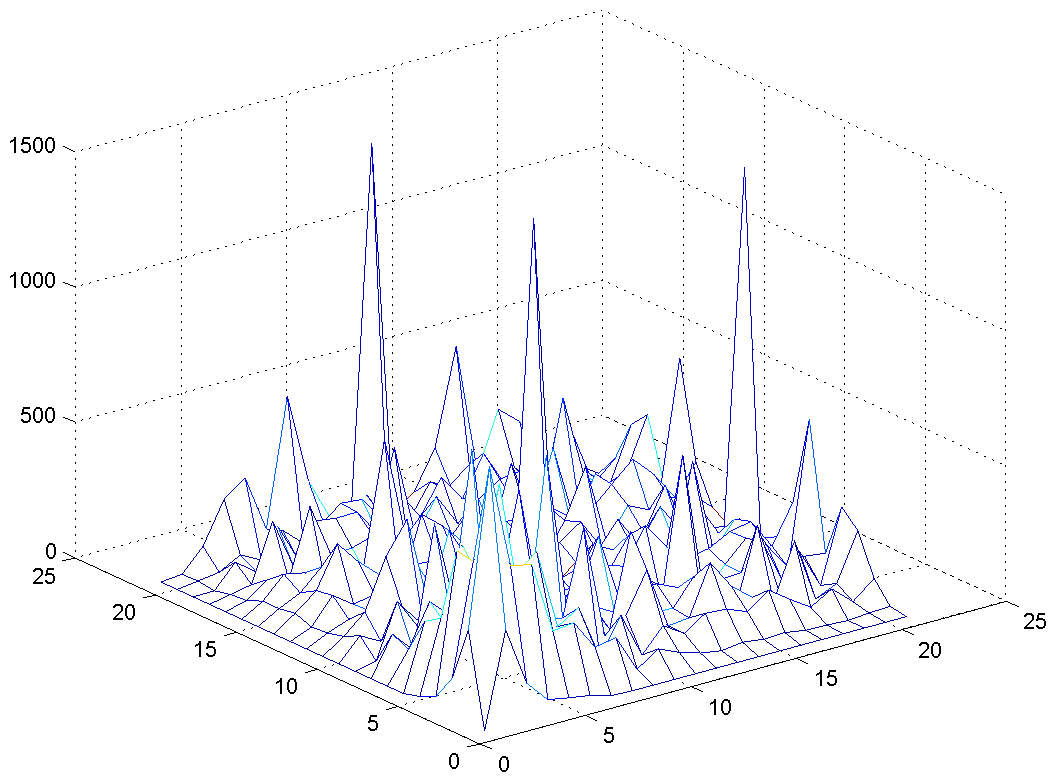
\includegraphics[scale = 0.3]{./images/examples/Rotatedtrigwno(15152020).png}}
                \caption{Αναπαράσταση περιστραμμένου τριγώνου με αριθμό επιπέδων κβάντισης: $\abs{\rho} = 15,\abs{\phi} = 15,\abs{\theta_1} = 20,\abs{\theta_2} = 20$}
        \end{subfigure}%
        \caption{Παράδειγμα με τρίγωνο}
\end{figure}
% =========================================================================================================================
% =========================================================================================================================

\begin{figure}
        \centering
        \begin{subfigure}[t]{0.3\textwidth}
                \centerline{
\includegraphics[scale = 0.5]{./images/examples/orthogwnio.png}}
                \caption{Ορθογώνιο}
        \end{subfigure}%
        ~
        \centering
        \begin{subfigure}[t]{0.3\textwidth}
                \centerline{
\includegraphics[scale = 0.5]{./images/examples/orthogwnio90.png}}
                \caption{Περιστραμμένο ορθογώνιο κατά 90 μοίρες}
        \end{subfigure}%
        \centering
        \begin{subfigure}[t]{0.3\textwidth}
                \centerline{
\includegraphics[scale = 0.5]{./images/examples/Rotatedorthogwnio.png}}
                \caption{Περιστραμμένο ορθογώνιο}
        \end{subfigure}%

        \centering
        \begin{subfigure}[b]{1\textwidth}
                \centerline{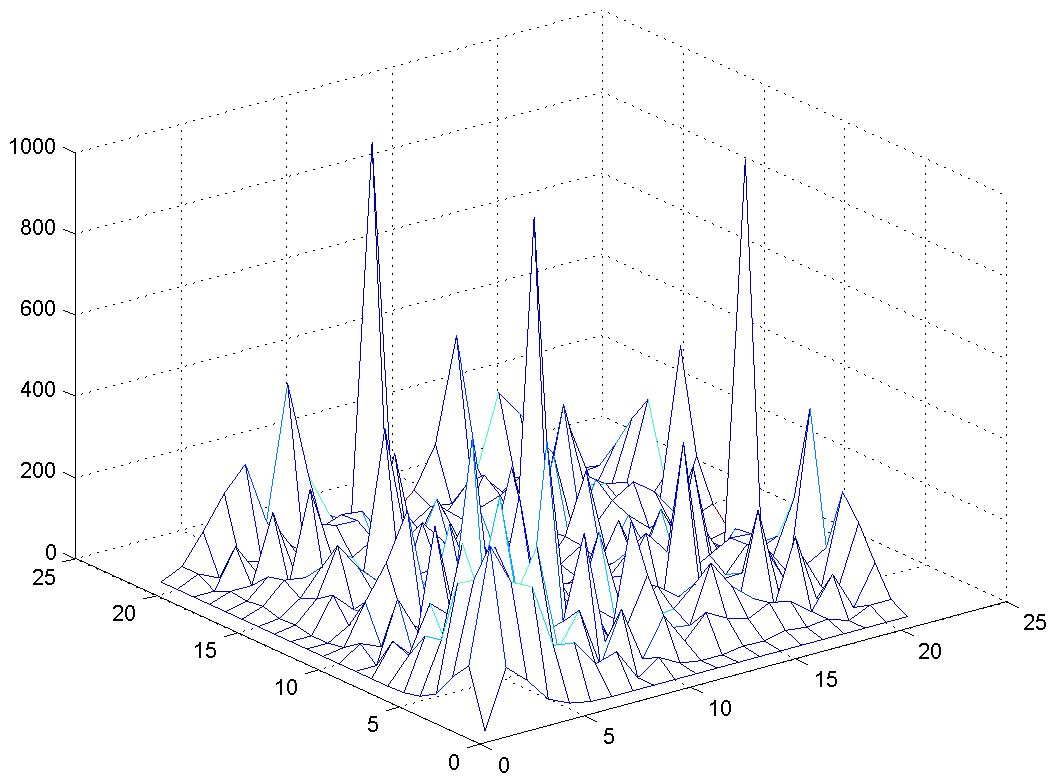
\includegraphics[scale = 0.3]{./images/examples/orthogwnio(15152020).png}}
                \caption{Αναπαράσταση ορθογωνίου με αριθμό επιπέδων κβάντισης: $\abs{\rho} = 15,\abs{\phi} = 15,\abs{\theta_1} = 20,\abs{\theta_2} = 20$}
        \end{subfigure}%
\end{figure}

\begin{figure}
\ContinuedFloat
        \centering
        \begin{subfigure}[b]{1\textwidth}
                \centerline{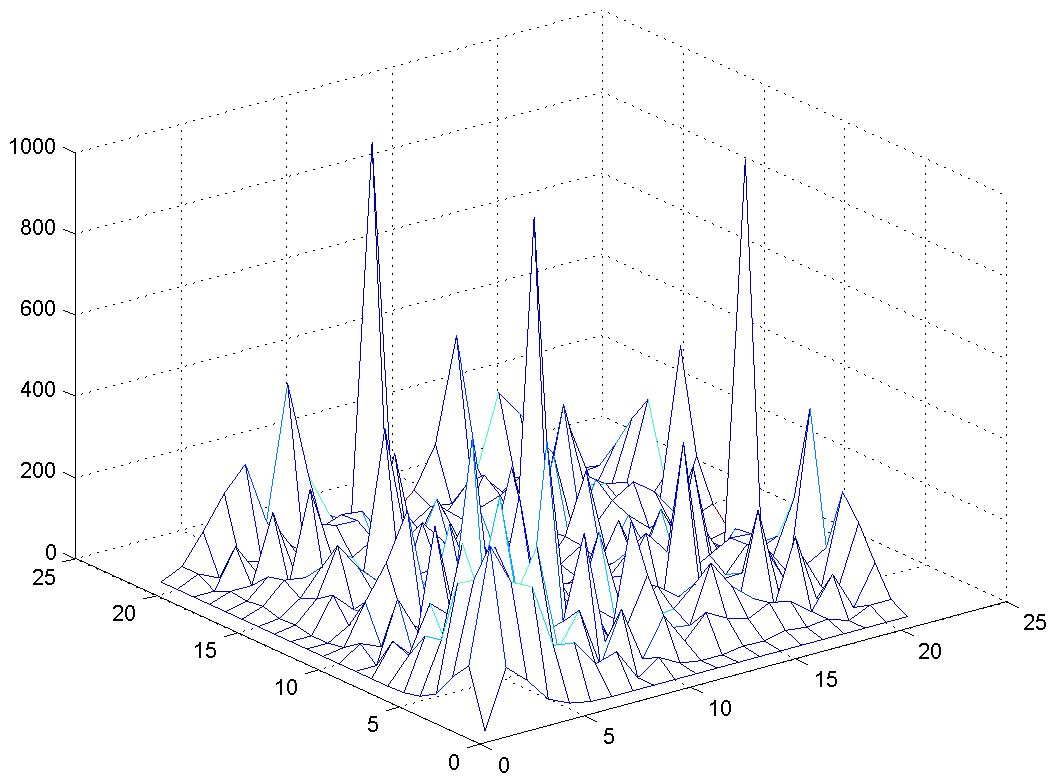
\includegraphics[scale = 0.3]{./images/examples/orthogwnio90(15152020).png}}
                \caption{Αναπαράσταση περιστραμμένου κατά 90 μοίρες ορθογωνίου με αριθμό επιπέδων κβάντισης: $\abs{\rho} = 15,\abs{\phi} = 15,\abs{\theta_1} = 20,\abs{\theta_2} = 20$}
        \end{subfigure}%

        \centering
        \begin{subfigure}[b]{1\textwidth}
                \centerline{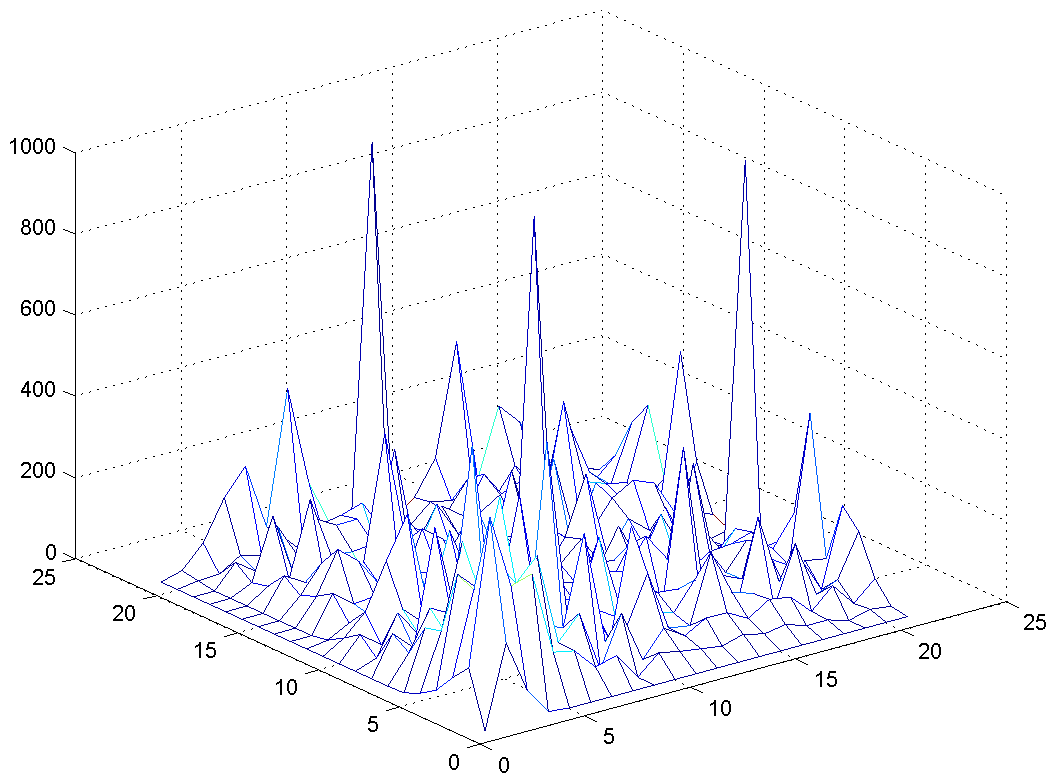
\includegraphics[scale = 0.3]{./images/examples/Rotatedorthogwnio(15152020).png}}
                \caption{Αναπαράσταση περιστραμμένου ορθογωνίου με αριθμό επιπέδων κβάντισης: $\abs{\rho} = 15,\abs{\phi} = 15,\abs{\theta_1} = 20,\abs{\theta_2} = 20$}
        \end{subfigure}%
        \caption{Παράδειγμα με ορθογώνιο}
        \label{fig:ex__rect}
\end{figure}
% =========================================================================================================================
% =========================================================================================================================

\paragraph*{}
Όπως φαίνεται από τα παραδείγματα των Σχημάτων \ref{fig:ex_rect}-\ref{fig:ex__rect}, οι αναπαραστάσεις της κάθε εικόνας και της αντίστοιχης περιστραμμένης είναι σχεδόν ίδιες. Υπάρχουν μικρές διαφοροποιήσεις, οι οποίες οφείλονται στην αλλοίωση που υφίστανται οι εικόνες κατά την περιστροφή τους. Όπως επιβεβαιώνεται, άλλωστε, στην περίπτωση του τριγώνου και του ορθογωνίου, οι αναπαραστάσεις για τις περιστραμμένες κατά 90 μοίρες εικόνες, όπου δεν υπάρχει αλλοίωση, ταυτίζονται \textit{απόλυτα}.

\paragraph*{}
Στη συνέχεια παρατίθενται τρεις αναπαραστάσεις του τετραγώνου (Σχήμα \ref{fig:rect}) για διαφορετικό αριθμό επιπέδων κβάντισης για τα $\rho,\phi,\theta_1,\theta_2$ (Σχήματα \ref{fig:diff}). Σε αυτές τις αναπαραστάσεις είναι πιο εμφανείς οι διαφορές. Παρόλα αυτά, μπορούμε να παρατηρήσουμε πως υπάρχει μια στοιχειώδης δομή για τη συγκεκριμένη εικόνα εισόδου, η οποία παραμένει σταθερή και στις τρεις περιπτώσεις.

\begin{figure}
        \centering
        \begin{subfigure}[b]{1\textwidth}
                \centerline{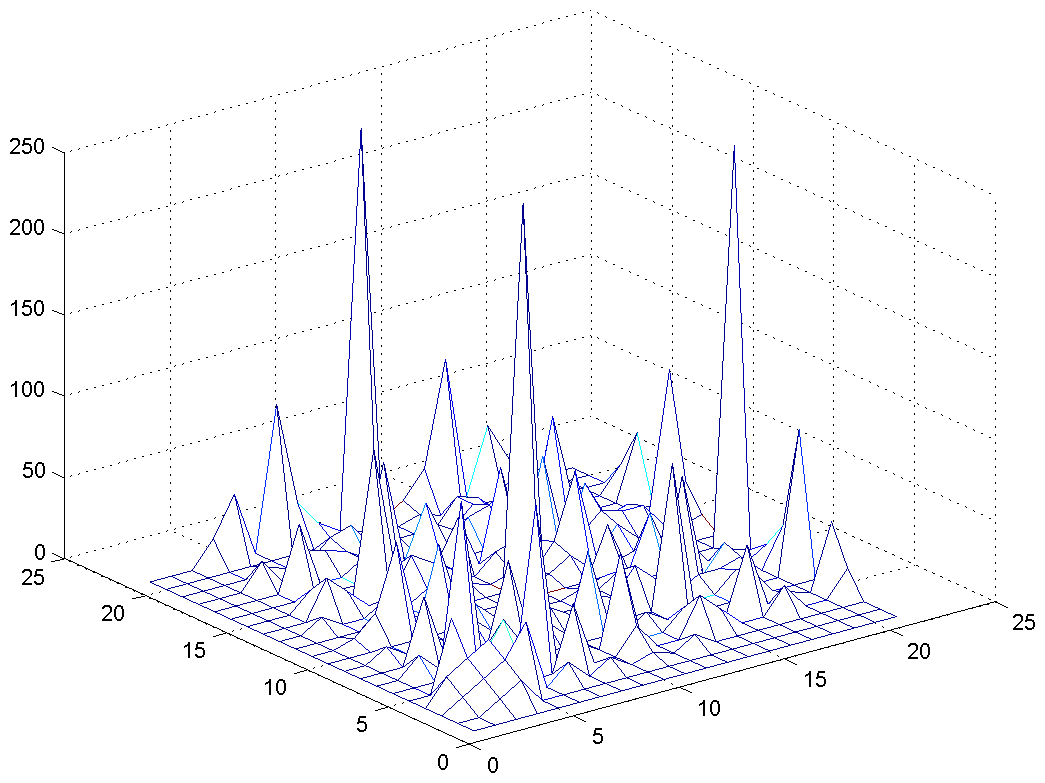
\includegraphics[scale = 0.35]{./images/examples/smallerTetragwno(15152020).png}}
                \caption{Αναπαράσταση τετραγώνου με αριθμό επιπέδων κβάντισης: $\abs{\rho} = 15,\abs{\phi} = 15,\abs{\theta_1} = 20,\abs{\theta_2} = 20$}
        \end{subfigure}

        \centering
        \begin{subfigure}[b]{1\textwidth}
                \centerline{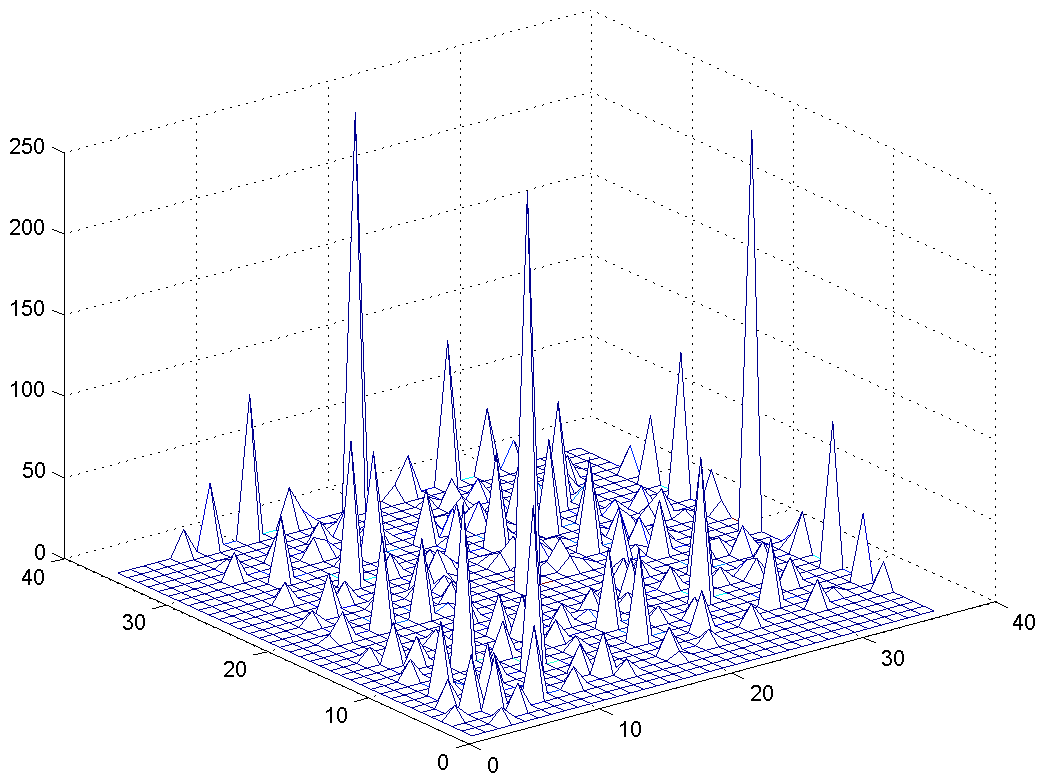
\includegraphics[scale = 0.35]{./images/examples/smallerTetragwno(25253535).png}}
                \caption{Αναπαράσταση τετραγώνου με αριθμό επιπέδων κβάντισης: $\abs{\rho} = 25,\abs{\phi} = 25,\abs{\theta_1} = 35,\abs{\theta_2} = 35$}
        \end{subfigure}
\end{figure}
\begin{figure}
\ContinuedFloat
        \centering
        \begin{subfigure}[b]{1\textwidth}
                \centerline{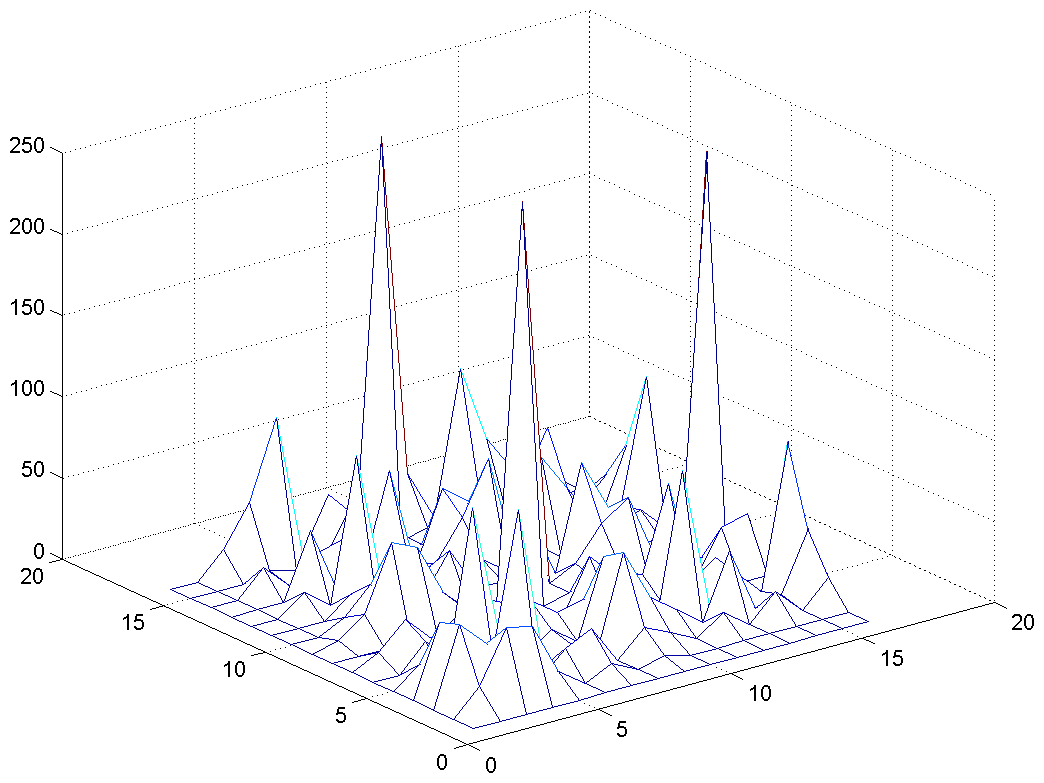
\includegraphics[scale = 0.35]{./images/examples/smallerTetragwno(551515).png}}
                \caption{Αναπαράσταση τετραγώνου με αριθμό επιπέδων κβάντισης: $\abs{\rho} = 5,\abs{\phi} = 5,\abs{\theta_1} = 15,\abs{\theta_2} = 15$}
        \end{subfigure}%
        \caption{Αναπαράσταση τετραγώνου για διαφορετικό αριθμό επιπέδων κβάντισης των $\rho,\phi,\theta_1,\theta_2$}
        \label{fig:diff}
\end{figure}

% =========================================================================================================================
% =========================================================================================================================

\section{Υλοποίηση Μοντέλου Bag of Words} \label{sec:real}
\paragraph*{}
Στην Παράγραφο \ref{sec:properties} σημειώθηκε πως, προκειμένου να ισχύουν οι ιδιότητες των συσχετίσεων, είναι απαραίτητο να μην υπάρχει απώλεια πληροφορίας της εικόνας, κατά το μετασχηματισμό της. Στα παραδείγματα της προηγούμενης παραγράφου, όπου παράχθηκε η αναπαράσταση τεχνητών εικόνων, λήφθηκε υπόψιν αυτή η απαίτηση. Έτσι, οι εικόνες τοποθετήθηκαν σε ένα μαύρο πλαίσιο και, όπως φαίνεται και στα αντίστοιχα σχήματα, κατά την περιστροφή τους δεν υπερέβαιναν αυτό το πλαίσιο και έτσι δεν αποκόπηκαν.

\paragraph*{}
Όταν, όμως, πρόκειται για πραγματικές εικόνες, είναι πολύ σπάνιο, αν όχι αδύνατο, αυτές να περιβάλλονται από πλαίσιο. Ακόμα πιο δύσκολο είναι να περιβάλλεται από μαύρο πλαίσιο κάποια συγκεκριμένη γειτονιά της εικόνας, για την οποία θα πρέπει να παραχθεί τοπικός περιγραφέας. Προκειμένου, λοιπόν να αναπαρασταθεί μια εικόνα μέσω του μοντέλου Bag of Words, χρησιμοποιώντας την προτεινόμενη αναπαράσταση για τη δημιουργία τοπικών περιγραφέων, θα πρέπει το πλαίσιο να προστεθεί στην εικόνα τεχνητά. Αυτό γίνεται με χρήση της γκαουσιανής συνάρτησης, συγκεκριμένα της διδιάστατης γκαουσιανής συνάρτησης.

\paragraph*{}
Ο τύπος για τη διδιάστατη γκαουσιανή συνάρτηση είναι:
\begin{equation}
f(x,y) = \alpha e^{-\left(\dfrac{(x-x_0)^2}{2\sigma_x^2}+\dfrac{(y-y_0)^2}{2\sigma_y^2}\right)}
\end{equation}
όπου $\alpha, x_0, y_0,\sigma_x, \sigma_y \in \mathbf{R}$. Όπως φαίνεται στο Σχήμα \ref{fig:2dbell}, το γράφημα της συνάρτησης έχει το σχήμα καμπάνας, είναι δηλαδή συμμετρικό και τείνει προς το μηδέν ασυμπτωτικά. Το $\alpha$ ορίζει το ύψος την επιφάνειας, τα $(x_0,y_0)$, ορίζουν το κέντρο και τα $(\sigma_x,\sigma_y)$ ορίζουν τα πλάτη της καμπάνας ως προς τους άξονες x και y αντίστοιχα. Συγκεκριμένα, όσο πιο μικρό είναι το $\sigma$, τόσο πιο γρήγορα φτάνουμε σε σχεδόν μηδενικές τιμές στην αντίστοιχη διάσταση.


\begin{figure}
\centerline{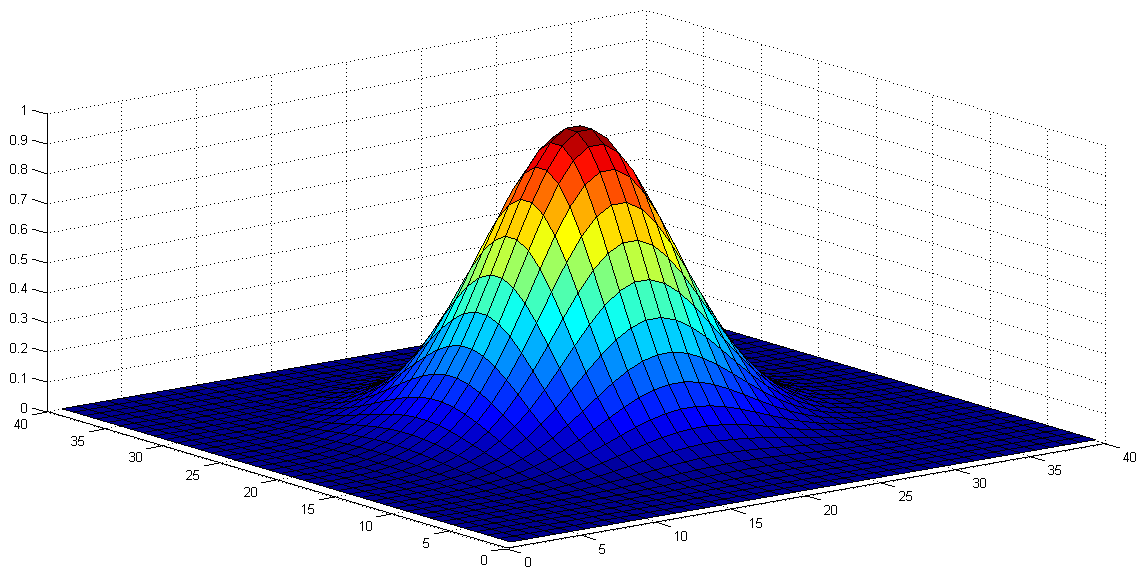
\includegraphics[scale=0.35]{./images/gauss2DCurve.png}}
\caption{Γράφημα της Γκαουσιανής συνάρτησης στις δύο διαστάσεις}
\label{fig:2dbell}
\end{figure}


\paragraph*{}
Προγραμματιστικά, όταν υπολογίζεται η γκαουσιανή συνάρτηση στις δύο διαστάσεις, στην ουσία αυτό που υπολογίζεται είναι ένας διδιάστατος πίνακας, του οποίου το στοιχείο που αντιστοιχεί στις συντεταγμένες $(x_0,y_0)$ περιέχει την τιμή $\alpha$ και οι τιμές των υπόλοιπων στοιχείων μειώνονται όσο μεγαλώνει η απόσταση από το $(x_0,y_0)$
\begin{wrapfigure}{r}{0.3\textwidth}
\centerline{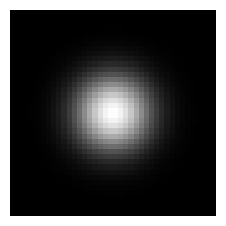
\includegraphics[scale=0.25]{./images/gauss2DImage.png}}
\caption{Γκαουσιανή συνάρτηση ως εικόνα}
\label{fig:2dbellimage}
\end{wrapfigure}
ακτινικά, έως ότου, σε μεγάλες αποστάσεις, σχεδόν να μηδενιστούν. Αν ο πίνακας αυτός αντιμετωπιστεί ως εικόνα\footnote{Ο πίνακας πρέπει να υποστεί κανονικοποίηση στη μονάδα, αν $\alpha \neq 1$.}, τότε το αποτέλεσμά είναι μία εικόνα αποχρώσεων του γκρι (grayscale), η οποία στο σημείο $(x_0,y_0)$ έχει τη μέγιστη φωτεινότητα (λευκό χρώμα), η οποία μειώνεται σταδιακά ανάλογα με την απόσταση από το σημείο $(x_0,y_0)$, μέχρι να φτάσει σε σχεδόν μηδενική φωτεινότητα (μαύρο χρώμα) (Σχ. \ref{fig:2dbellimage}). Ο πίνακας που μόλις περιγράφηκε μπορεί να πολλαπλασιαστεί στοιχείο προς στοιχείο με τα στοιχεία κάποιας εικόνας (έγχρωμης ή/και grayscale) και, ανάλογα με τα επιλεγμένα $\sigma_x,\sigma_y$ και $(x_0,y_0)$, να μείνει εμφανές κάποιο κομμάτι της εικόνας και γύρω από το κομμάτι αυτό η εικόνα να μαυρίσει (Σχήμα \ref{fig:peppers}). Ιδιαίτερη προσοχή χρειάζεται στην περίπτωση έγχρωμων εικόνων, όπου θα πρέπει ο πίνακας της γκαουσιανής να πολλαπλασιαστεί ξεχωριστά με κάθε χρωματική συνιστώσα της εικόνας. Για παράδειγμα, αν χρησιμοποιείται το χρωματικό μοντέλο RGB (Red Green Blue), τότε η εικόνα αναπαρίσταται από έναν πίνακα τριών διαστάσεων. Οι δυο πρώτες διαστάσεις αφορούν στη θέση κάθε σημείου πάνω στην εικόνα και η τρίτη διάσταση (με μήκος τρία) αφορά στη χρωματική συνιστώσα. Είναι δηλαδή στην ουσία, τρεις ξεχωριστοί διδιάστατοι πίνακες ίδιας διάστασης με την εικόνα, όπου ο κάθε πίνακας περιέχει τις τιμές της κάθε ξεχωριστής χρωματικής συνιστώσας. Σε αυτήν την περίπτωση θα πρέπει ο πίνακας της γκαουσιανής συνάρτησης να πολλαπλασιαστεί ξεχωριστά με καθέναν από τους τρεις πίνακες των χρωμάτων και το αποτέλεσμα αυτών των πολλαπλασιασμών θα συνθέτει την τελική εικόνα. 
\begin{figure}[!t]
        \centering
        \begin{subfigure}[b]{0.5\textwidth}
                \centerline{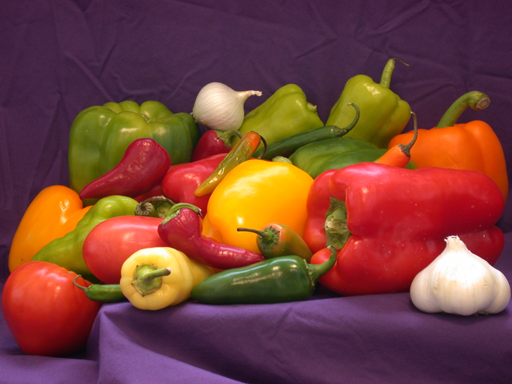
\includegraphics[scale = 0.4]{./images/peppers.png}}
        \end{subfigure}%
		~
        \centering
        \begin{subfigure}[b]{0.5\textwidth}
                \centerline{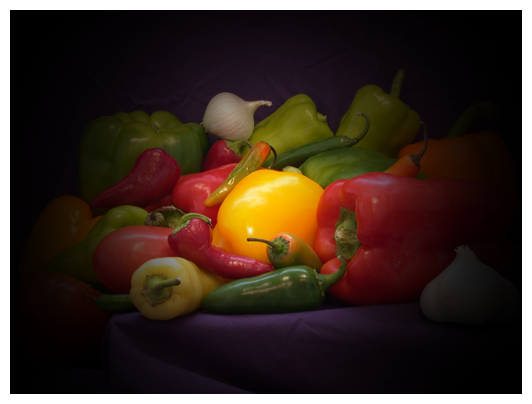
\includegraphics[scale = 0.4]{./images/peppers1.png}}
        \end{subfigure}%


        \centering
        \begin{subfigure}[t]{0.5\textwidth}
                \centerline{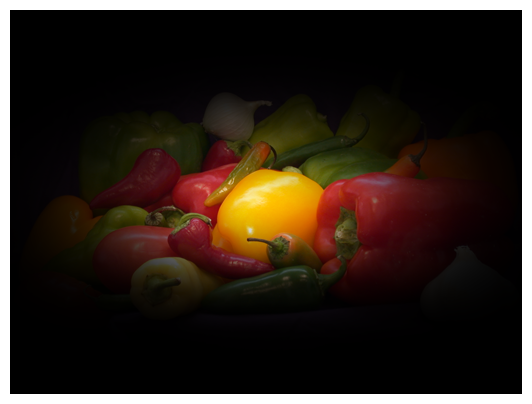
\includegraphics[scale = 0.4]{./images/peppers2.png}}
        \end{subfigure}%
        ~
        \centering
        \begin{subfigure}[t]{0.5\textwidth}
                \centerline{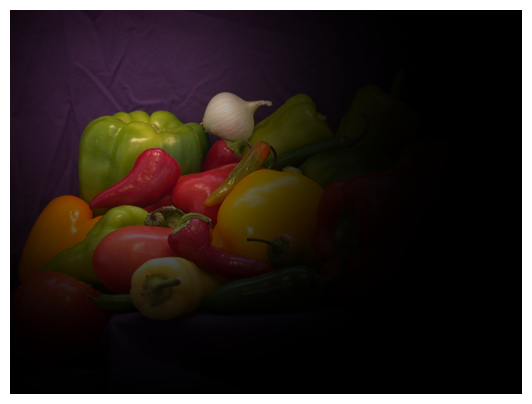
\includegraphics[scale = 0.4]{./images/peppers4.png}}
        \end{subfigure}%
        \caption{Εικόνα πολλαπλασιασμένη με γκαουσιανή συνάρτηση με διαφορετικά $\sigma_x,\sigma_y$ και $(x_0,y_0)$}
        \label{fig:peppers}
\end{figure}

\paragraph*{}
Έτσι, για την παραγωγή των τοπικών περιγραφέων πάνω στο πλέγμα που έχει εφαρμοστεί στην εικόνα, αυτό που γίνεται είναι να πολλαπλασιάζεται η εικόνα με την γκαουσιανή, η οποία είναι κεντραρισμένη κάθε φορά στον κόμβο του οποίου ο περιγραφέας πρέπει να δημιουργηθεί. Τα $\sigma_x,\sigma_y$ επιλέγονται κατάλληλα, έτσι ώστε η γειτονιά που μένει εμφανής να έχει το μέγεθος που έχει επιλεχθεί. Στο Σχήμα \ref{fig:lena} φαίνεται η διαδικασία που περιγράφηκε, όπου το κέντρο της γειτονιάς επιλέχθηκε με γραφικό τρόπο.


\begin{figure}[!b]
        \centering
        \begin{subfigure}[t]{0.5\textwidth}
                \centerline{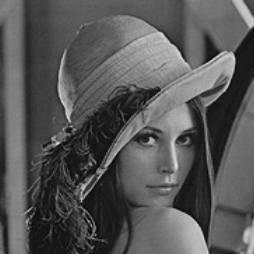
\includegraphics[scale = 0.7]{./images/examples/lena.jpg}}
                \caption{Αρχική εικόνα}
        \end{subfigure}%
		~
        \centering
        \begin{subfigure}[t]{0.5\textwidth}
                \centerline{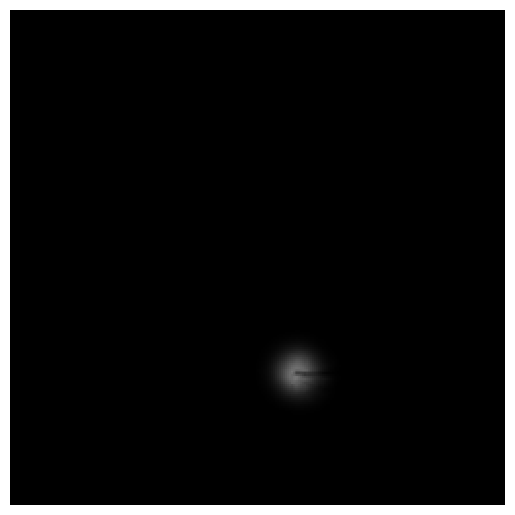
\includegraphics[scale = 0.35]{./images/examples/pointNo3afterGaussian.png}}
                \caption{Μετά τον πολλαπλασιασμό με τη Γκαουσιανή συνάρτηση}
        \end{subfigure}%

        \centering
        \begin{subfigure}[t]{0.8\textwidth}
                \centerline{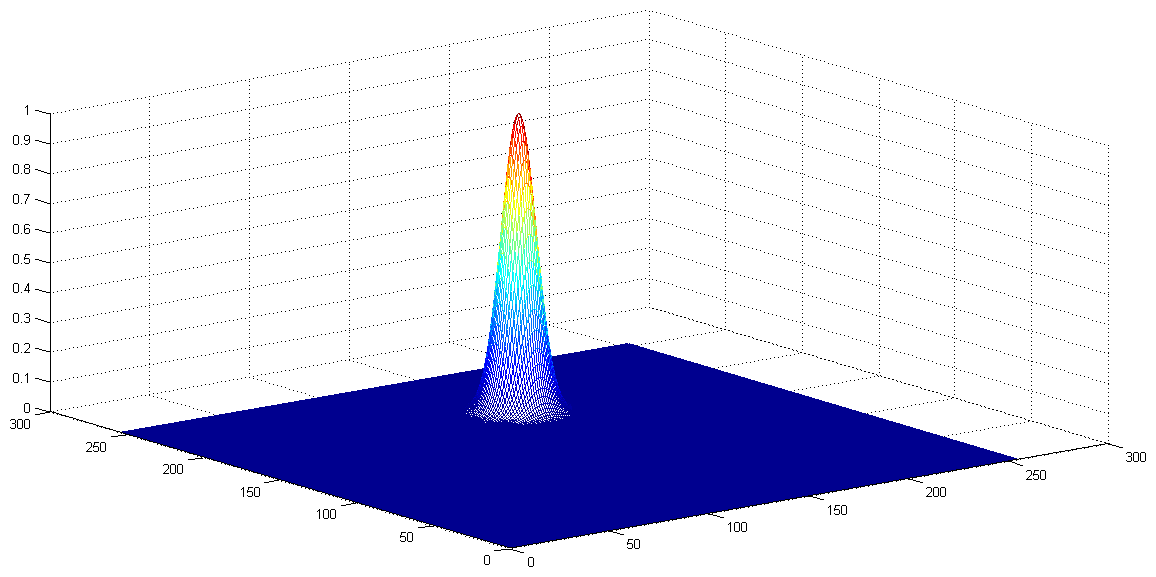
\includegraphics[scale = 0.25]{./images/examples/gaussianOfPointNo3.png}}
                \caption{Γκαουσιανή συνάρτηση κεντραρισμένη στο σημείο ενδιαφέροντος}
        \end{subfigure}%
        ~
        \centering
        \begin{subfigure}[t]{0.2\textwidth}
                \centerline{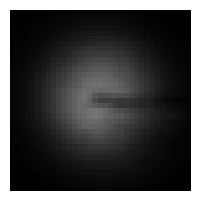
\includegraphics[scale = 0.2]{./images/examples/pointNo3cropped.png}}
                \caption{Τελική εικόνα}
        \end{subfigure}%
        \caption{Παράδειγμα με πραγματική εικόνα}
        \label{fig:lena}
\end{figure}
